\documentclass[border=4pt]{standalone}
% Preámbulo común de las figuras. Cada figura es un documento standalone
% que se compila a SVG con scripts/build_figures.sh
\usepackage[utf8]{inputenc}
\usepackage{amsmath}
\usepackage{tikz}
\usepackage[american, siunitx]{circuitikz}
\usetikzlibrary{arrows.meta,calc,decorations.pathmorphing,patterns}
\tikzset{
  >={Stealth[length=2.2mm]},
  eje/.style={->, thin},
  hilo/.style={thick},
}
% Paleta común: tonos medios legibles sobre fondo claro
\definecolor{azul}{RGB}{31,94,168}
\definecolor{rojo}{RGB}{192,57,43}
\definecolor{verde}{RGB}{39,128,73}
\definecolor{naranja}{RGB}{211,120,30}
\definecolor{morado}{RGB}{125,60,152}

\begin{document}
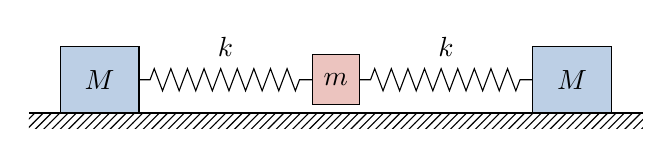
\begin{tikzpicture}[scale=1.0]
  \fill[pattern=north east lines] (-0.4,-0.62) rectangle (7.4,-0.42);
  \draw[thick] (-0.4,-0.42) -- (7.4,-0.42);
  \fill[azul!30] (0,-0.42) rectangle (1,0.42); \draw (0,-0.42) rectangle (1,0.42);
  \fill[rojo!30] (3.2,-0.32) rectangle (3.8,0.32); \draw (3.2,-0.32) rectangle (3.8,0.32);
  \fill[azul!30] (6,-0.42) rectangle (7,0.42); \draw (6,-0.42) rectangle (7,0.42);
  \node at (0.5,0) {$M$}; \node at (3.5,0) {$m$}; \node at (6.5,0) {$M$};
  \draw[decorate, decoration={zigzag, segment length=6pt, amplitude=4pt, pre length=4pt, post length=4pt}] (1,0) -- node[above=5pt]{$k$} (3.2,0);
  \draw[decorate, decoration={zigzag, segment length=6pt, amplitude=4pt, pre length=4pt, post length=4pt}] (3.8,0) -- node[above=5pt]{$k$} (6,0);
\end{tikzpicture}
\end{document}
